\documentclass{article}
\usepackage{josuamathheader}

\newcommand{\ggT}{\operatorname{ggT}}

\usepackage{tkz-euclide}

\begin{document}
\section*{Aufgabe 1}
\begin{enumerate}[(a)]
    \item Betrachte eine Matrix
    \[
        \overline{A} =  \begin{pmatrix}
            \overline{a} & \overline{b}\\
            \overline{c} & \overline{d}
        \end{pmatrix} \in \operatorname{SL}(\Z/N\Z)
    \]
    Es gilt $ad - bc \equiv 1 \mod N$, d.h. $m \coloneqq \ggT(a,b) | 1 \mod N$ und damit $\ggT(m, N) = 1$.
    Mit Benutzung des euklidischen Algorithmus erhalten wir die Existenz von $u, v$ mit $ua + vb = m$ und $sm + rN = 1$.
    Dann gilt für Vertreter $a,b,c,d\in \Z$
    \[
        \begin{pmatrix}
            a & b\\
            c & d
        \end{pmatrix} \cdot
        \overbrace{
        \underbrace{\begin{pmatrix}
            u & -b\\
            v & a
        \end{pmatrix}}_{\in \operatorname{SL}_2(\Z)} \cdot
        \underbrace{\begin{pmatrix}
            s & N\\
            -r & m
        \end{pmatrix}}_{\in \operatorname{SL}_2(\Z)}}^{B}
        = \begin{pmatrix}
            m & 0\\
            * & *
        \end{pmatrix} \cdot \begin{pmatrix}
            s & N\\
            -r & m
        \end{pmatrix}
        = \begin{pmatrix}
            sm & Nm\\
            * & *
        \end{pmatrix} \eqqcolon M
    \]
    Betrachten wir also alle Matrizen $\mod N$, so erhalten wir $M \in \operatorname{SL}_2(\Z/n\Z)$ und durch Rechnung folgt
    \[
        \begin{pmatrix}
            sm & Nm\\
            * & *
        \end{pmatrix} \equiv \begin{pmatrix}
            sm + rN & 0\\
            * & * 
        \end{pmatrix} \equiv \begin{pmatrix}
            1 & 0\\
            * & * 
        \end{pmatrix} \overset{!}{\equiv} \begin{pmatrix}
            1 & 0\\
            * & 1
        \end{pmatrix} \mod N
    \]
    Diese Matrix besitzt ein Urbild $C$ in $\operatorname{SL}_2(\Z)$, d.h. es gilt $\operatorname{mod}(N)(C) = \begin{pmatrix}
        1 & 0\\
        * & 1
    \end{pmatrix} \equiv M$.
    $$\operatorname{mod}(N)(C \cdot B^{-1}) = \operatorname{mod}(N)(C) \cdot \operatorname{mod}(N)(B^{-1}) = \overline{M} \cdot \overline{B^{-1}} = \overline{ABB^{-1}} = \overline{A}$$
    Damit haben wir für ein beliebiges $\overline{A} \in \operatorname{SL}_2(\Z/N\Z)$ ein Urbild $C \cdot B^{-1} \in \operatorname{SL}_2(\Z)$ konstruiert, insbesondere ist $\operatorname{mod}(N)$ surjektiv.
    \item Wir berechnen die Anzahl der Möglichkeiten für eine Matrix $M \in \operatorname{GL}_2(\Z/p^\nu\Z)$.
    In die erste Spalte können wir jede Kombination $(x,y)$ von zwei Elementen $x,y \in \Z/p^\nu\Z$ schreiben, solange $p \not | \ggT(x,y)$. Sonst folgt nämlich $p | \det(M)$, also $\det M \equiv 0 \mod p^\nu$, was im Widerspruch zur Regularität von $M$ steht.
    Es gibt für die erste Spalte also insgesamt $(p^\nu)^2$ Möglichkeiten, von denen wir wieder $(p^\nu)^2/p^2$ abziehen müssen, da für jedes $p^2$-te Paar $(x,y)$ gilt $p | x \land p | y$.
    Insgesamt gibt es also $p^{2\nu} \cdot (1 - p^{-2})$ Möglichkeiten für die erste Spalte.
    Die zweite Spalte muss so gewählt werden, dass keine Linearkombination (wobei $l$ invertierbar sein muss) aus erster und zweiter Spalte einen durch $p$ teilbaren größten gemeinsamen Teiler besitzt.
    Die Menge aller Spalten, die nicht vorkommen dürfen, ist gegeben durch
    \begin{align*}
        \left\{\begin{pmatrix}
            b\\d
        \end{pmatrix} \big| l \cdot \begin{pmatrix}
            b\\d
        \end{pmatrix} - k \cdot \begin{pmatrix}
            a\\c
        \end{pmatrix} = \begin{pmatrix}
            mp\\np
        \end{pmatrix} \Leftrightarrow l \cdot \begin{pmatrix}
            b\\d
        \end{pmatrix} = \begin{pmatrix}
            mp\\np
        \end{pmatrix} + k \cdot \begin{pmatrix}
            a\\c
        \end{pmatrix}\right\}
    \end{align*} mit $l$ invertierbar.
    Betrachten wir diese Forderung modulo $p$, so erhalten wir
    \begin{align*}
        l \cdot \begin{pmatrix}
            b\\d
        \end{pmatrix} &\equiv k \cdot \begin{pmatrix}
            a\\c
        \end{pmatrix}\\
        \begin{pmatrix}
            b\\d
        \end{pmatrix} &\equiv l^{-1}k \cdot \begin{pmatrix}
            a\\c
        \end{pmatrix}\\
    \end{align*}
    Es sind also die $p$ Äquivalenzklassen $l^{-1}k = 0,1,\dots, p-1$ ausgeschlossen. Jede dieser Äquivalenzklassen besitzt $p^{2\nu}/p^2$ Elemente. Insgesamt sind damit $p \cdot p^{2\nu}/p^2$ Möglichkeiten für die zweite Spalte ausgeschlossen.
    Es bleiben also $p^{2\nu} \cdot (1 - p^{-1})$ Möglichkeiten, sodass insgesamt die Behauptung folgt.
    \item Betrachte den surjektiven Gruppenhomomorphismus
    \[
        \det \operatorname{GL}_2(\Z/p^\nu \Z) \to (\Z/p^\nu\Z)^\times
    \]
    Es gilt $\ker \det = \operatorname{SL}_2(\Z/p^\nu \Z)$ und daher
    \[
        |\operatorname{SL}_2(\Z/p^\nu \Z)| = |\operatorname{GL}_2(\Z/p^\nu \Z)| / |(\Z/p^\nu\Z)^\times| = p^{4\nu}(1-p^{-1})(1 - p^{-2})/(p^\nu (1 - p^{-1})) = p^{3\nu}(1- p^{-2}).
    \]
    \item Für alle Kongruenzgruppen $\Gamma$ gilt: $\exists N$ mit $\Gamma(N) \subset \Gamma$. Da $\Gamma(N)$ endlichen Index hat, folgt die Existenz von Matrizen $A_1, \dots A_r$ mit 
    \[
        \operatorname{SL}_2(\Z) = A_1 \Gamma(N) + \dots + A_r \Gamma(N) \subset A_1 \Gamma + \dots + A_r \Gamma.
    \]
    Folglich existieren auch höchstens $r < \infty$ Nebenklassen zu $\Gamma$ und damit ist $[\operatorname{SL}_2(\Z) \colon \Gamma] < \infty$.
\end{enumerate}
\section*{Aufgabe 2}
\begin{enumerate}[(a)]
    \item Wir zeigen die drei Bedingungen aus Definition 1.21.
    \begin{enumerate}[(i)]
        \item Möbiustransformationen sind stetig auf $\mathbb{H}$. Insbesondere ist also $M \circ F$ wieder zusammenhängend und, weil die Umkehrabbildung ebenfalls stetig ist, auch abgeschlossen.
        \item Durch Anwenden einer Möbiustransformation $M$ auf einen Punkt $z$ ändert sich nichts an der Äquivalenzklasse von $z$ bezüglich der Operation der Möbiustransformationen.
        \item Der Rand von $F$ ist homöomorph zur $S^1$. $M \circ F$ und das Bild des Inneren $M\circ F^\circ$ sind zusammenhängend.
        Das Bild des Randes $\partial F$ ist wieder homöomorph zur $S^1$. Aus topologischen Gründen wird nun $\partial F$ auf $\partial M \circ F$ abgebildet. Es gilt nämlich $M \circ F^\circ = M \circ F \setminus \underbrace{M \circ \partial F}_{\simeq S^1}$. Ist nun $M \circ \partial F$ nicht $\partial M\circ F$, so teilt $M \circ \partial F$ den topologischen Raum $M \circ F$ in zwei nicht wegzusammenhängende Komponenten, Widerspruch.

        Sei also $A\langle y\rangle = z$ mit $y, z \in (M \circ F)^ \circ = M\circ F^\circ$.
        Dann gilt $M^{-1} A M \langle M^{-1}\langle y\rangle \rangle = M^{-1}\langle z \rangle$ mit $M^{-1}\langle y \rangle, M^{-1}\langle z \rangle \in F^\circ$.
        Diese beiden Punkte müssen aber entweder identisch oder inäquivalent sein, da sie beide aus dem Inneren eines Fundamentalbereichs stammen.
        Also folgt $M^{-1}A M = \operatorname{id} \Leftrightarrow A = \operatorname{id}$ und je zwei Punkte $y,z \in (M \circ F)^\circ$ sind entweder identisch oder inäquivalent.
    \end{enumerate}
    \item Siehe Abbildung \ref{fig:fundamentalbereich}
    \begin{figure}[h!]
        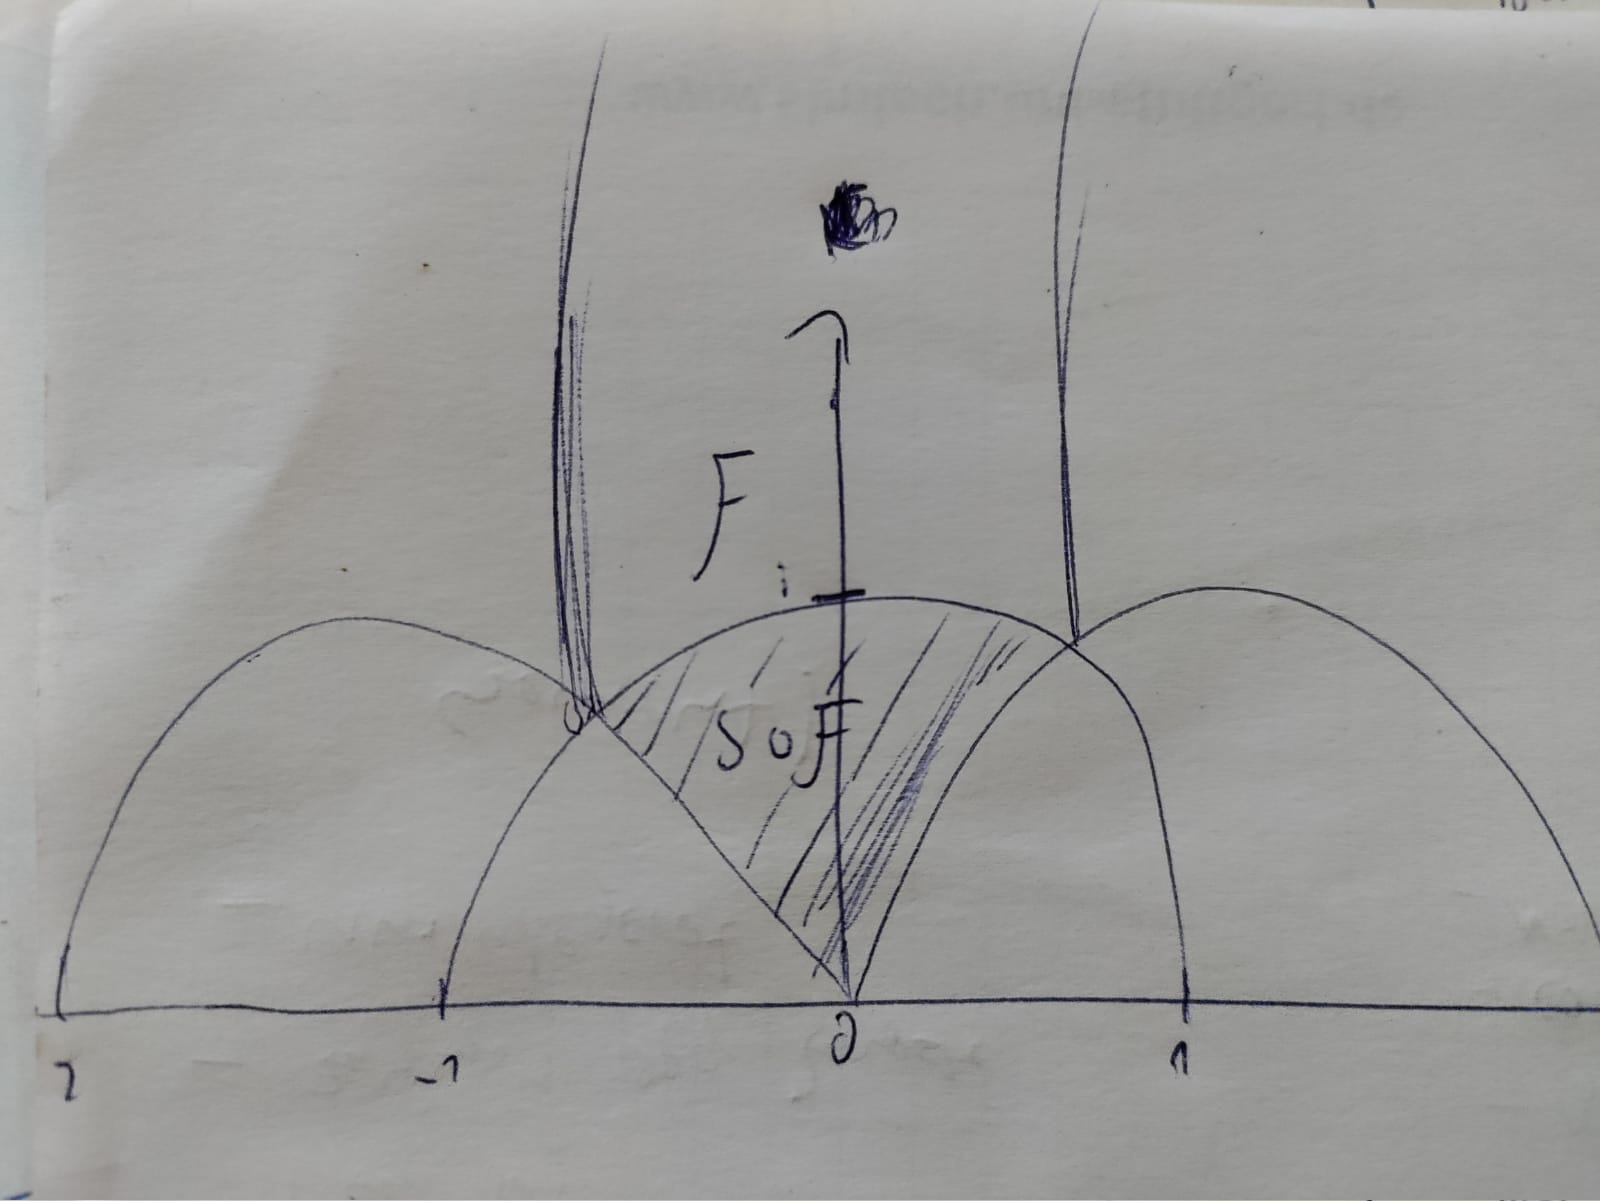
\includegraphics[width=\textwidth]{fundamentalbereich.jpeg}
        \caption{Skizze Fundamentalbereich}
        \label{fig:fundamentalbereich}
    \end{figure}
\end{enumerate}
\section*{Aufgabe 3}
\begin{enumerate}[(a)]
    \item Sei $M = \begin{pmatrix}
        a & b\\c& d
    \end{pmatrix} \in \Gamma_0(p)$.
    Dann gilt $M\langle 0 \rangle = \frac{b}{d}$.
    Wegen $p | c$ und $\ggT(c,d) \not | p$ (sonst ist $M$ nicht regulär) folgt $p \not | d$.
    Außerdem gilt $M\langle \infty \rangle = \frac{a}{c}$.
    Wir erhalten also zwei Spitzenklassen:
    \[
        \begin{cases}
            \frac{r}{q} \sim 0 & p \not | q,\\
            \frac{r}{q} \sim \infty & p | q.
        \end{cases}  
    \]
    mit der Konvention $p | 0$ und $\infty = \frac{1}{0}$.
    Die Vereinigung beider Spitzenklassen ist also bereits $\Q \cup \infty$, es kann keine weiteren Spitzenklassen geben.
    \item Analog zur a) erhalten wir $M\langle 0 \rangle = \frac{b}{d}$ mit $p \not | d$ und $M\langle \infty \rangle = \frac{a}{c}$ mit $p^2|c$. Insbesondere sind die beiden Spitzenklassen von $0$ und $\infty$ disjunkt.
    Wir erhalten
    \[
        M\langle -\frac{1}{kp} \rangle = \frac{-\frac{a}{kp}+b}{-\frac{c}{kp}+d} = \frac{-a + kbp}{-c + kbp}
    \]
    Angenommen, $$M\langle -\frac{1}{kp} \rangle = 0 \implies -a = kbp \implies p | a.$$ Dann wären aber $a$ und $c$ durch $p$ teilbar und somit auch die Determinante, im Widerspruch zu $M \in \Gamma_0(p)$.
    Angenommen, $$M\langle -\frac{1}{kp} \rangle = \infty \implies -c = kdp \implies p^2 | kdp \implies p|d.$$ Dann wären aber $c$ und $d$ durch $p$ teilbar und somit auch die Determinante, im Widerspruch zu $M \in \Gamma_0(p)$.
    Angenommen,
    \begin{align*}
        M\langle -\frac{1}{kp} \rangle &= -\frac{1}{lp}\\
        \frac{-a + kbp}{-c + kdp} &= - \frac{1}{lp}\\
        a - kbp &= \frac{-c + kdp}{lp}\\
        alp - lkbp^2 &= -c + kdp\\
        al - kd &= \frac{-c}{p} + klbp\\
        \intertext{$p^2 | c$, also handelt es sich hierbei um eine ganzzahlige Gleichung}
        al - kd &= \left(\frac{-c}{p^2} + klb\right)p
    \end{align*}
    Wir folgern durch Betrachtung modulo $p$, dass $p | (al - kd)$.
    Ziel wäre es jetzt noch, zu zeigen, dass $k = l$ gelten muss. Dann hätte man die Disjunktheit der Spitzenklassen gezeigt.
    Außerdem müsste man dann noch zeigen, dass die Vereinigung der Spitzenklassen $\Q \cup \{\infty\}$ ergibt.
\end{enumerate}
\end{document}